\documentclass{article}
% PACKAGES %
\usepackage[english]{} % Sets the language
\usepackage[margin=2cm]{geometry} % Sets the margin size
\usepackage{fancyhdr} % Allows creation of headers
\usepackage{xcolor} % Allows the use of color in text
\usepackage{float} % Allows figures and tables to be floats
\usepackage{appendix}
\usepackage{amsmath} % Enhanced math package prepared by the American Mathematical Society
	\DeclareMathOperator{\sech}{sech} % Include sech
\usepackage{amssymb} % AMS symbols package
\usepackage{mathrsfs}% More math symbols
\usepackage{breqn} % Allows line breaking in math mode
\usepackage{cancel} % Allows math strikethroughs to show cancellations
\usepackage{bm} % Allows you to use \bm{} to make any symbol bold
\usepackage{bbold} % Allows more bold characters
\usepackage{verbatim} % Allows you to include code snippets
\usepackage{setspace} % Allows you to change the spacing between lines at different points in the document
\usepackage{parskip} % Allows you alter the spacing between paragraphs
\usepackage{multicol} % Allows text division into multiple columns
\usepackage{units} % Allows fractions to be expressed diagonally instead of vertically
\usepackage{booktabs,multirow,multirow} % Gives extra table functionality
\usepackage[final]{pdfpages} % Allows pdfs to be imported
\usepackage{hyperref} % Allows hyperlinks in the document
\usepackage{rotating} % Allows tables to be rotated
\usepackage{graphicx} % Enhanced package for including graphics/figures
	% Set path to figure image files
	\graphicspath{ {fig/} }
\usepackage{listings} % for including text files
	\lstset{basicstyle=\ttfamily\scriptsize,
        		  keywordstyle=\color{blue}\ttfamily,
        	  	  stringstyle=\color{red}\ttfamily,
          	  commentstyle=\color{gray}\ttfamily,
          	 }		
\newcommand{\tab}{\-\hspace{1cm}}

\newcommand{\p}{\partial}
\newcommand{\ppt}{\frac{\p}{\p t}}
\newcommand{\grad}{\vec{\nabla}}

\newcommand{\Xs}{\Sigma}
\newcommand{\xs}{\sigma}

\newcommand{\Oov}{\frac{1}{v}}

\newcommand{\pos}{\vec{r}}
\newcommand{\cur}{\vec{J}}
\newcommand{\Oh}{\hat{\Omega}}

\newcommand{\intfp}{\int_{4\pi}}
\newcommand{\intzi}{\int_0^{\infty}}


\newcommand{\rt}{(\pos,t)}
\newcommand{\rE}{(\pos,E)}
\newcommand{\rEO}{(\pos,E,\Oh)}
\newcommand{\rEt}{(\pos,E,t)}
\newcommand{\rEtprime}{(\pos,E',t)}
\newcommand{\rEOprime}{(\pos,E',\Oh')}
\newcommand{\rOt}{(\pos,\Oh,t)}
\newcommand{\rOtprime}{(\pos,\Oh',t)}
\newcommand{\rEOt}{(\pos,E,\Oh,t)}
\newcommand{\rEOtprime}{(\pos,E',\Oh',t)}
\newcommand{\EO}{(E,\Oh)}
\newcommand{\EOprime}{(E',\Oh')}
\newcommand{\EOt}{(E,\Oh,t)}



% Create a header w/ Name & Date
\pagestyle{fancy}
\rhead{\textbf{Mitch Negus} \; 10/20/2017}

\begin{document}
\thispagestyle{empty}

{\bf {\large {NE250 Homework {3} \hfill Mitch Negus\\
		\hspace*{\fill} 10/20/2017\\ }}}
		
		
		
%%%%%%%%%%%%%%%%%%%%%%%%%%%%%%%%%% PROBLEM 1 %%%%%%%%%%%%%%%%%%%%%%%%%%%%%%%%%%

\section*{Problem 1}

We are given
\begin{align*}
\left[\Oh \cdot \nabla + \Xs_t(E) \right] \psi\rEO &= \intfp d\Oh' \intzi dE' \Xs_s(E',\Oh' \rightarrow E,\Oh)\psi\rEOprime \\
&+ \frac{1}{k}\frac{\chi(E)}{4\pi} \intzi dE' \nu(E') \Xs_f(E') \intfp d\Oh' \psi\rEOprime.
\end{align*}

If we have isotropic scattering (and no cross section spatial dependence), then $\Xs_s(E',\Oh' \rightarrow E,\Oh) = \Xs_s(E' \rightarrow E)$.
\begin{align*}
\left[\Oh \cdot \nabla + \Xs_t(E) \right] \psi\rEO &= \intzi dE' \Xs_s(E' \rightarrow E) \intfp d\Oh' \psi\rEOprime \\
&+ \frac{1}{k}\frac{\chi(E)}{4\pi} \intzi dE' \nu(E') \Xs_f(E') \intfp d\Oh' \psi\rEOprime.
\end{align*}

Now, we let $\psi\rEO = \psi_0\EO\exp(i \Oh \cdot \vec{B})$. Noting that $\Oh \cdot \vec{B} = \mu|\vec{B}|$, the equation for $\psi$ can be substituted into our equation above to yield
\begin{align*}
\left[\Oh \cdot \nabla + \Xs_t(E) \right] \psi_0\EO\exp(i \mu|\vec{B}|) &= \intzi dE' \Xs_s(E' \rightarrow E) \intfp d\Oh' \psi_0\EOprime\exp(i \mu|\vec{B}|) \\
&+ \frac{1}{k}\frac{\chi(E)}{4\pi} \intzi dE' \nu(E') \Xs_f(E') \intfp d\Oh' \psi_0\EOprime\exp(i \mu|\vec{B}|).
\end{align*}

Rearranging to solve for $k$,
\begin{align*}
\left[\Oh \cdot \nabla + \Xs_t(E) \right] \psi_0\EO\exp(i \mu|\vec{B}|) &- \intzi dE' \Xs_s(E' \rightarrow E) \intfp d\Oh' \psi_0\EOprime\exp(i \mu|\vec{B}|) \\
& = \frac{1}{k}\frac{\chi(E)}{4\pi} \intzi dE' \nu(E') \Xs_f(E') \intfp d\Oh' \psi_0\EOprime\exp(i \mu|\vec{B}|).
\end{align*}
$$ k = \frac{\frac{\chi(E)}{4\pi} \intzi dE' \nu(E') \Xs_f(E') \intfp d\Oh' \psi_0\EOprime\exp(i \mu|\vec{B}|)}{\left[\Oh \cdot \nabla + \Xs_t(E) \right] \psi_0\EO\exp(i \mu|\vec{B}|) - \intzi dE' \Xs_s(E' \rightarrow E) \intfp d\Oh' \psi_0\EOprime\exp(i \mu|\vec{B}|)} $$
...



%%%%%%%%%%%%%%%%%%%%%%%%%%%%%%%%%% PROBLEM 2 %%%%%%%%%%%%%%%%%%%%%%%%%%%%%%%%%%

\section*{Problem 2}

The one-group diffusion equation can be derived from the neutron transport equation using Fick's Law ($\cur(\pos) = -D(\pos)\nabla \phi$). 

If we have no external source, the one-group transport equation is 
\begin{align*}
\Oov \frac{\p \phi\rOt}{\p t} + \Omega \cdot \nabla \phi \rOt + \Xs_t \psi\rOt = \intfp d\Oh' \Xs_s(\Oh' \rightarrow \Oh) \psi\rOtprime + \frac{\nu\Xs_f}{4\pi} \intfp d\Oh' \psi\rOtprime
\end{align*}
This would then be integrated over angle, under the assumption that the angular flux is only weakly dependent on angle. Additionally, we assume that the scattering is azimuthally symmetric, and so $\intfp d\Oh \, \Xs_s(\Oh' \rightarrow \Oh) = \intfp d\Oh \, \Xs_s(\Oh' \cdot \Oh) = \Xs_s$.
\begin{align*}
\intfp d\Oh \left[ \Oov \frac{\p \psi\rOt}{\p t} + \Oh \cdot \nabla \psi \rOt + \Xs_t \psi\rOt \right] &= \intfp d\Oh \bigg[ \intfp d\Oh' \Xs_s(\Oh' \rightarrow \Oh) \psi\rOtprime \\
&+ \frac{\nu\Xs_f}{4\pi} \intfp d\Oh' \psi\rOtprime \bigg]
\end{align*}
\begin{align*}
\Oov \frac{\p \phi\rt}{\p t} + \nabla \cdot \cur\rt + \Xs_t \phi\rt &=\Xs_s \phi\rt + \nu\Xs_f \phi\rt
\end{align*}
\begin{align*}
\Oov \frac{\p \phi\rt}{\p t} -D(\pos)\nabla \phi\rt + \Xs_t \phi\rt &=\Xs_s \phi\rt + \nu\Xs_f \phi\rt
\end{align*}
Now, we can assume our reactor is approximately steady state, so the time dependence vanishes, and we note that since we have only one group, the only scattering reactions which contribute to our neutron gain are $(n,xn)$ reactions. The equation reduces to
$$ -D(\pos)\nabla \phi(\pos) + \Xs_t \phi(\pos) =\sum_{n=2}^{\infty}x \Xs_{(n,xn)} \phi(\pos) + \nu\Xs_f \phi(\pos) $$
$$ -D(\pos)\nabla \phi(\pos) + \Xs_t \phi(\pos) - \sum_{n=2}^{\infty}x \Xs_{(n,xn)} \phi(\pos) = \nu\Xs_f \phi(\pos) $$
For small deviations of $k_{\textit{eff}}$, this can be
$$ -D(\pos)\nabla \phi(\pos) + \Xs_t \phi(\pos) - \sum_{n=2}^{\infty}x \Xs_{(n,xn)} \phi(\pos) = \frac{1}{k}\nu\Xs_f \phi(\pos) $$
$$\boxed{ k = \frac{\nu\Xs_f \phi(\pos)}{-D(\pos)\nabla \phi(\pos) + \Xs_t \phi(\pos) - \sum_{n=2}^{\infty}x \Xs_{(n,xn)} \phi(\pos)} }$$



%%%%%%%%%%%%%%%%%%%%%%%%%%%%%%%%%% PROBLEM 3 %%%%%%%%%%%%%%%%%%%%%%%%%%%%%%%%%%

\section*{Problem 3}

Define $G$ as the ratio between total power generated, $P$, to fusion power generated, $P_F$.
$$ G \equiv \frac{P}{P_F} $$
As a ratio, this is also equivalent to the ratio between total energy created, $E$, to fusion energy created, $E_F$.
$$ G  = \frac{E}{E_F} $$
Since we are told that energy contributions from non-fission reactions are neglible. This suggests that the total energy is simply the sum of the fission energy produced, $E_f$, and fusion energy produced, $E_F$. 
$$ G = \frac{E_F + E_f}{E_F} = 1 + \frac{E_f}{E_F}$$
Each DT fusion reaction produces 17.6 MeV of energy and one neutron for triggering fission in the blanket, so $E_F = 17.6\textsl{n}_0$ MeV, where \textsl{n}_0 is the number of neutrons produced from fusion. With an 80\% probability of triggering an $(n,2n)$ reaction in beryllium, the average fusion event results in approximately 1.8 neutrons eventually reaching the blanket. If we again take the fact that even negative energy-contributions from non-fission reactions are neglible, as well as the fact that no fusion neutrons leak from the system, then we can assume that each fusion neutron produces at least one fission event or elastically scatters. Mathematically,
$$ \Xs_f + \Xs_s = \Xs_t ,$$
and the probability of a "first strike" fission event is
$$ \text{P}(F) = \frac{\Xs_f}{\Xs_t}. $$
From this, we can determine the number of neutrons in the first generation after interaction in the blanket, $\textsl{n}_1$ as the number of neutrons produced in those "first strike" fissions plus the number of neutrons remaining after scattering
$$ \textsl{n}_1 = 1.8(\nu \text{P}(f) + \text{P}(s))\textsl{n}_0 = 1.8\left(\nu \frac{\Xs_f}{\Xs_t} + \frac{\Xs_s}{\Xs_t}\right)\textsl{n}_0 .$$
Some of these neutrons may now leak out of the system, however, so in general the number of neutrons in generation $t$, given as $\textsl{n}_t$, will obey the relation
$$ \textsl{n}_t = k_{\text{eff}}\textsl{n}_{t-1} ,$$
where $k_{\textit{eff}}$ now also accounts for leakage.
The total fission energy produced by a single generation of fusion events and the ensuing multiplication and fission (assuming the energy produced in a single fission event to be about 200 MeV) will be
$$ E_f = 200 \left(\frac{\Xs_f}{\Xs_t}\right)\left(1.8\textsl{n}_0 + \sum_{t=1}^{\infty} n_t \right) \text{MeV} $$
$$ E_f = 200 \left(\frac{\Xs_f}{\Xs_t}\right)\left(1.8\textsl{n}_0 + \sum_{t=1}^{\infty}k_{\textit{eff}}\textsl{n}_{t-1} \right) \text{MeV} $$
$$ E_f = 200 \left(\frac{\Xs_f}{\Xs_t}\right)\left(1.8\textsl{n}_0 + 1.8\sum_{t=1}^{\infty}k_{\textit{eff}}^{t-1}\textsl{n}_0 \right) \text{MeV} $$
$$ E_f = 360 \left(\frac{\Xs_f}{\Xs_t}\right)\textsl{n}_0 \left(1  + \sum_{t=1}^{\infty}k_{\textit{eff}}^{t-1} \right) \text{MeV} $$
$$ E_f = 360 \left(\frac{\Xs_f}{\Xs_t}\right)\textsl{n}_0 \sum_{t=0}^{\infty}k_{\textit{eff}}^{t-1} \text{ MeV} $$
Altogether, we find
$$ G = 1 + \frac{360 \left(\frac{\Xs_f}{\Xs_t}\right)\textsl{n}_0 \sum_{t=0}^{\infty}k_{\textit{eff}}^{t-1} \text{ MeV}}{17.6 \textsl{n}_0 \text{ MeV}} $$
$$\boxed{ G = 1 + 20.5 \left(\frac{\Xs_f}{\Xs_t}\right) \sum_{t=0}^{\infty}k_{\textit{eff}}^{t-1} }$$



%%%%%%%%%%%%%%%%%%%%%%%%%%%%%%%%%% PROBLEM 4 %%%%%%%%%%%%%%%%%%%%%%%%%%%%%%%%%%

\section*{Problem 4}

\subsection*{\textit{a.})}

We are given the matrix:

$$\begin{bmatrix}
1 	&	1	&	-1	&	3	\\
1	&	2	&	-4	&	-2	\\
2	&	1	&	1	&	5	\\
-1	&	0	&	-2	&	-4	\end{bmatrix}$$

The inverse, $\textbf{A}^{-1}$ of a square matrix, $\textbf{A}$,  is equal to the adjugate of the matrix, $\textbf{A}^{\dagger}$ divided by the determinant of $\textbf{A}$. 

$$ \textbf{A}^{-1} = \frac{\textbf{A}^{\dagger}}{\det{\textbf{A}}} $$

The adjugate of a square matrix, $\textbf{A}^{\dagger}$, is the transpose of the cofactor matrix, $\textbf{C}_{\textbf{A}}$.

$$ \textbf{A}^{\dagger} = \textbf{C}_{\textbf{A}}^T $$

The cofactor of a square matrix, $\textbf{C}_{\textbf{A}}$ is the signed matrix of minors, $\textbf{M}_{\textbf{A}}$.

$$ \textbf{C}_{\textbf{A},ij} = (-1)^{i+j} \ \textbf{M}_{\textbf{A}} $$

The minor of matrix element $\textbf{A}_{ij}$ is the determinant of submatrix formed with the rows and columns other than $i$ and $j$.

We can use this all together to find the inverse of $\textbf{A}$. The matrix given, however, has a determinant of zero, and so is \underline{not invertible}.

(see attached Jupyter notebook for full calculations)


\subsection*{\textit{b.})}

We are given the matrix:

$$\begin{bmatrix}
3 	&	-1	\\
-1	&	3	\end{bmatrix}$$

and we know that the eigenvalue $\lambda$ and eigenvector $\vec{v}$ obey the rule

$$\begin{bmatrix}
3 	&	-1	\\
-1	&	3	\end{bmatrix}\vec{v} = \lambda \vec{v}$$

Equivalently, 

$$\left(\begin{bmatrix}
3 	&	-1	\\
-1	&	3	\end{bmatrix} - \lambda\mathbb{1}\right)\vec{v} = 0$$

We want the non-trivial solution to this equation, when $\vec{v} \neq \vec{0}$. $\vec{v} = \vec{0}$ when $\left(\begin{bmatrix}
3 	&	-1	\\
-1	&	3	\end{bmatrix} - \lambda\mathbb{1}\right)$ is invertible, so we will instead assert that $\left(\begin{bmatrix}
3 	&	-1	\\
-1	&	3	\end{bmatrix} - \lambda\mathbb{1}\right)$ is not invertible. By definition, this means 

$$ \det\left(\begin{bmatrix}
3 	&	-1	\\
-1	&	3	\end{bmatrix} - \lambda\mathbb{1}\right) = 0 $$

or 

$$ \det\begin{bmatrix}
3-\lambda	&	-1	\\
-1	&	3-\lambda	\end{bmatrix} = 0 $$

We can solve this now for lambda:


\begin{align*}
(3-\lambda)^2 - (-1)^2 &= 0 \\
9 - 6\lambda + \lambda^2 - 1 &= 0 \\
8 - 6\lambda + \lambda^2 &= 0 \\
\end{align*}

and using the quadratic formula we find

$$ \lambda = \frac{-(-6) \pm \sqrt{(-6)^2 - 4(8)}}{2} $$
$$ \lambda = \frac{6 \pm \sqrt{36 - 32}}{2} $$
$$ \lambda = \frac{6 \pm 2}{2} $$
$$ \lambda = 3 \pm 1$$

$$\boxed{ \lambda = 2, 4 }$$

We can use this eigenvalue to solve for $\vec{v}$. 

$$\begin{bmatrix}
1 	&	-1	\\
-1	&	1	\end{bmatrix}\vec{v} = 0 \ \text{ and } \ 
\begin{bmatrix}
-1 	&	-1	\\
-1	&	-1	\end{bmatrix}\vec{v} = 0 $$ 

This gives the equations

$$ \lambda = 2: \begin{cases} v_1 - v_2 = 0 \\
                              v_2 - v_1 = 0 \end{cases}
\qquad \lambda = 4: \begin{cases}  -v_1 - v_2 = 0 \end{cases} $$

For $\boxed{ \lambda = 2, \ \vec{v} = \begin{bmatrix}v_0 \\ v_0\end{bmatrix} }$, and for $\boxed{ \lambda = 4, \ \vec{v} = \begin{bmatrix}v_0 \\ -v_0\end{bmatrix} }$.



%%%%%%%%%%%%%%%%%%%%%%%%%%%%%%%%%% PROBLEM 5 %%%%%%%%%%%%%%%%%%%%%%%%%%%%%%%%%%

\section*{Problem 5}

In problem 4 we stated that the inverse, $\textbf{A}^{-1}$, of a square matrix, $\textbf{A}$,  is equal to the adjugate of the matrix, $\textbf{A}^{\dagger}$ divided by the determinant of $\textbf{A}$.

$$ \textbf{A}^{-1} = \frac{\textbf{A}^{\dagger}}{\det{\textbf{A}}} $$

We can manipulate this expression to find

$$ (\det{\textbf{A}})\mathbb{1} = \textbf{A}^{\dagger}\textbf{A} $$

Since we are looking for a self-adjugate matrix, $\textbf{A}^{\dagger} = \textbf{A}$, and 

$$ (\det{\textbf{A}})\mathbb{1} = \textbf{A}^2 .$$

Then, taking the square root of both sides,

$$ \left(\sqrt{\det{\textbf{A}}}\right)\mathbb{1} = \textbf{A} .$$

$$ \textbf{A} = \begin{bmatrix} a & b & c \\
                                d & e & f \\
                                g & h & i \end{bmatrix} =
                \begin{bmatrix} \sqrt{\det{\textbf{A}}} & 0 & 0 \\
                                0 & \sqrt{\det{\textbf{A}}} & 0 \\
                                0 & 0 & \sqrt{\det{\textbf{A}}} \end{bmatrix}. $$
                
$$ a = e = i = \sqrt{\det{\textbf{A}}} $$
$$ \textbf{A} = \begin{bmatrix} a & 0 & 0 \\
                                0 & a & 0 \\
                                0 & 0 & a \end{bmatrix} = $$
and

$$ \det{\textbf{A}} = a \begin{vmatrix} a & 0 \\ 0 & a \end{vmatrix} $$
$$ \det{\textbf{A}} = a (a^2) $$
$$ \det{\textbf{A}} = a^3 .$$

We know that $a = \sqrt{\det{\textbf{A}}}$, so
$$ a = \sqrt{a^3} $$
$$ a = a^{\frac{3}{2}} $$
$$ a = 1 $$
$$\boxed{ \textbf{A} = \mathbb{1} }$$

We can furthermore use the functions defined in the previous problem to show that $\textbf{A}$ and  $\textbf{A}^{\dagger}$ are equal when found through the cofactor method.

(see attached Jupyter notebook for full calculations)



%%%%%%%%%%%%%%%%%%%%%%%%%%%%%%%%%% PROBLEM 6 %%%%%%%%%%%%%%%%%%%%%%%%%%%%%%%%%%

\section*{Problem 6}

From Duderstadt and Hamilton, we can "define the operator $M^{\dagger}$ adjoint to the operator $M$ as that operator $M^{\dagger}$ for which
$$ (M^{\dagger}f,g) = (f,Mg) ,"$$
where parentheses denote the inner product such that
$$ (f,g) \equiv \int_{a_i}^{a_f} f^*(\pos)g(\pos) dx $$
for the interval $[a_i,a_f]$, and $f^*$ is the complex conjugate of $f$.
Now, we wish to show that $L \equiv \frac{d^2}{dx^2}$ is self adjoint,
$$ L = L^{\dagger} ,$$
when $f$ has a derivative everywhere, is symmetric about the origin, and obeys Dirichlet boundary conditions ($f(\pm a) = 0$), all on the closed interval $[-a,a]$.

If $L = L^{\dagger}$, then
\begin{align*}
(Lf,g)	&= (f,Lg) \\
		&= \int_{-a}^{a} f^*(x) Lg(x) \, dx \\
		&= \int_{-a}^{a} f^*(x) \frac{d^2g(x)}{dx^2} \, dx \\
\end{align*}
Using integration by parts once,
\begin{align*}
(Lf,g)	&= \left[f^*(x)\frac{dg(x)}{dx}\right]_{-a}^{a} - \int_{-a}^{a} \frac{dg(x)}{dx}\frac{df^*(x)}{dx} \, dx \\
\end{align*}
and again,
$$ (Lf,g) = \left[f^*(x)\frac{dg(x)}{dx}\right]_{-a}^{a} - \left[\frac{dg(x)}{dx}f^*(x)\right]_{-a}^{a} + \int_{-a}^{a} g(x)\frac{d^2f^*(x)}{dx^2} \, dx $$
gives us an equation that can be manipulated into the form of our original operator definition.
$$ (Lf,g) = f^*(a)\frac{dg(x)}{dx}\bigg|_{a} - f^*(-a)\frac{dg(x)}{dx}\bigg|_{-a} - \frac{dg(x)}{dx}\bigg|_{a}f^*(a) + \frac{dg(x)}{dx}\bigg|_{-a}f^*(-a) + \int_{-a}^{a} g(x)\frac{d^2f^*(x)}{dx^2} \, dx $$
Given our boundary conditions, $f(\pm a) = 0$, we can say that $f^*(\pm a) = 0$. Then,
\begin{align*}
(Lf,g)	&= \int_{-a}^{a} g(x)\frac{d^2f^*(x)}{dx^2} \, dx \\
		&= \int_{-a}^{a} \frac{d^2f^*(x)}{dx^2}g(x) \, dx \\
		(Lf,g)	&= (Lf,g)
\end{align*}
\tab\tab$\square$



%%%%%%%%%%%%%%%%%%%%%%%%%%%%%%%%%% PROBLEM 7 %%%%%%%%%%%%%%%%%%%%%%%%%%%%%%%%%%

\section*{Problem 7}

The diffusion equation describing this one-dimensional slab is (assuming constant diffusion coefficients and cross sections in each region)

\text{Fuel:}
$$ -D_F\frac{d^2}{dx^2}\phi(x) + \Xs_{a,F}\phi(x) = 0 $$

\text{Moderator:}
$$ -D_M\frac{d^2}{dx^2}\phi(x) + \Xs_{a,M}\phi(x) = S_0 $$

\text{Boundary Conditions:}
\begin{align*}
\phi_F(a) 	&= \phi_M(a)  & \text{(interface condition)} \\
\cur_M\left(\pm\frac{a}{2} \pm b\right)	&= 0 \quad (\text{or }\phi\left(\pm \frac{a}{2} \pm \tilde{b}\right)=0) & \text{(effective vacuum boundary condition)}\\
\frac{d}{dx}\phi_F\bigg|_{x=0}	&= 0 & \text{(symmetry condition)}
\end{align*}

We can then solve for the flux in each region. In the fuel,
$$ \frac{d^2}{dx^2}\phi_F(x) - \frac{1}{L_F^2}\phi(x) = 0 $$

where $L_F = \sqrt{\frac{D_F}{\Xs_{a,F}}}$. The solution to this differential equation is of the form
$$ \phi_F(x) = A_1 e^{\frac{x}{L_F}} + A_2 e^{-\frac{x}{L_F}} $$

Using our symmetry condition,
$$ \frac{d\phi_F(x)}{dx} = \frac{A_1}{L_F}e^{\frac{x}{L_F}} - \frac{A_2}{L_F} e^{-\frac{x}{L_F}} $$
$$ 0 = \frac{A_1}{L_F} - \frac{A_2}{L_F} $$
$$ A_1 = A_2 = A_F $$
Then $\phi(x)$ becomes
$$ \phi_F(x) = A_F \left(e^{\frac{x}{L_F}} + e^{-\frac{x}{L_F}}\right) $$
$$ \phi_F(x) = A_F \cosh\left(\frac{x}{L_F}\right) $$


In the moderator,
$$ \frac{d^2}{dx^2}\phi(x) - \frac{1}{L_M^2}\phi(x) = -\frac{S_0}{D_M} $$
where $L_M = \sqrt{\frac{D_M}{\Xs_{a,M}}}$. Like the solution in the fuel, the homogeneous solution to this differential equation is of the form
$$ \phi_{\text{h}}(x) = A_3 e^{\frac{x}{L_M}} + A_4 e^{-\frac{x}{L_M}} $$
while the particular solution is
$$ \phi_{\text{p}}(x) = \frac{S_0 L_M^2}{D_M} .$$
The general solution in the moderator is then,
$$ \phi_M(x) = A_3 e^{\frac{x}{L_M}} + A_4 e^{-\frac{x}{L_M}} + \frac{S_0 L_M^2}{D_M} $$
Imposing our boundary conditions,
$$ \phi_M(\frac{a}{2}+\tilde{b}) = A_3 e^{\frac{\frac{a}{2}+\tilde{b}}{L_M}} + A_4 e^{-\frac{\frac{a}{2}+\tilde{b}}{L_M}} + \frac{S_0 L_M^2}{D_M} = 0 $$
and 
$$ \phi_M(-\frac{a}{2}-\tilde{b}) = A_3 e^{-\frac{\frac{a}{2}+\tilde{b}}{L_M}} + A_4 e^{\frac{\frac{a}{2}+\tilde{b}}{L_M}} + \frac{S_0 L_M^2}{D_M} = 0 .$$
Then,
$$ A_3 e^{\frac{\frac{a}{2}+\tilde{b}}{L_M}} + A_4 e^{-\frac{\frac{a}{2}+\tilde{b}}{L_M}} + \frac{S_0 L_M^2}{D_M} = A_3 e^{-\frac{\frac{a}{2}+\tilde{b}}{L_M}} + A_4 e^{\frac{\frac{a}{2}+\tilde{b}}{L_M}} + \frac{S_0 L_M^2}{D_M} $$
and
$$ A_3 = A_4 = A_M$$
so
$$ \phi_M(x) = A_M \left( e^{\frac{x}{L_M}} + e^{-\frac{x}{L_M}} \right) + \frac{S_0 L_M^2}{D_M} $$
Again, 
$$ \phi_M(\frac{a}{2}+\tilde{b}) = 0 = A_M \left( e^{\frac{\frac{a}{2}+\tilde{b}}{L_M}} + e^{-\frac{\frac{a}{2}+\tilde{b}}{L_M}} \right) + \frac{S_0 L_M^2}{D_M}$$
$$ A_M = \frac{-S_0 L_M^2}{D_M \left( e^{\frac{\frac{a}{2}+\tilde{b}}{L_M}} + e^{-\frac{\frac{a}{2}+\tilde{b}}{L_M}}\right)} $$
Then,
$$ \phi_M(x) = \left(\frac{-S_0 L_M^2}{D_M \left( e^{\frac{\frac{a}{2}+\tilde{b}}{L_M}} + e^{-\frac{\frac{a}{2}+\tilde{b}}{L_M}}\right)}\right) \left( e^{\frac{x}{L_M}} + e^{-\frac{x}{L_M}} \right) + \frac{S_0 L_M^2}{D_M} $$
$$ \phi_M(x) = \frac{-S_0 L_M^2 \cosh\left(\frac{x}{L_M}\right)}{D_M \cosh\left(\frac{\frac{a}{2}+\tilde{b}}{L_M}\right)} + \frac{S_0 L_M^2}{D_M} $$
$$\boxed{ \phi_M(x) = \frac{S_0 L_M^2}{D_M}\left( 1 - \frac{\cosh\left(\frac{x}{L_M}\right)}{\cosh\left(\frac{\frac{a}{2}+\tilde{b}}{L_M}\right)}\right) }.$$

Taking this back to our equation for $\phi_F(x)$, and using our interface condition,
$$ \phi_F(a) = \phi_M(a) $$
$$ A_F \cosh\left(\frac{a}{L_F}\right) = \frac{S_0 L_M^2}{D_M}\left( 1 - \frac{\cosh\left(\frac{a}{L_M}\right)}{\cosh\left(\frac{\frac{a}{2}+\tilde{b}}{L_M}\right)}\right) $$
$$ A_F = \frac{S_0 L_M^2}{D_M \cosh\left(\frac{a}{L_F}\right)}\left( 1 - \frac{\cosh\left(\frac{a}{L_M}\right)}{\cosh\left(\frac{\frac{a}{2}+\tilde{b}}{L_M}\right)}\right) $$

$$\boxed{ \phi_F(x) = \frac{S_0 L_M^2 \cosh\left(\frac{x}{L_F}\right)}{D_M \cosh\left(\frac{a}{L_F}\right)}\left( 1 - \frac{\cosh\left(\frac{a}{L_M}\right)}{\cosh\left(\frac{\frac{a}{2}+\tilde{b}}{L_M}\right)}\right) }.$$

If we define $f_s$ as the average flux in the fuel to the average flux in the cell, we find
$$ f_s = \frac{\frac{1}{a}\int_{-a/2}^{a/2} \phi_F(x) \, dx}{\frac{1}{a+2b}\int_{-b}^{b} \phi(x) \, dx} .$$
We can recognize, due to symmetry, that
$$ f_s = \frac{\frac{2}{a}\int_{0}^{a/2} \phi_F(x) \, dx}{\frac{2}{a+2b}\int_{0}^{b} \phi(x) \, dx} .$$
Then, we can write the denominator as
$$ f_s = \frac{\frac{2}{a}\int_{0}^{a/2} \phi_F(x) \, dx}{\frac{2}{a+2b}\left[\int_{0}^{a/2} \phi_F(x) \, dx + \int_{a/2}^{b} \phi_M(x) \, dx \right]} $$
Substituting our flux expressions,
$$ f_s = \frac{\frac{2}{a}\int_{0}^{a/2} \frac{S_0 L_M^2 \cosh\left(\frac{x}{L_F}\right)}{D_M \cosh\left(\frac{a}{L_F}\right)}\left( 1 - \frac{\cosh\left(\frac{a}{L_M}\right)}{\cosh\left(\frac{\frac{a}{2}+\tilde{b}}{L_M}\right)}\right) dx}{\frac{2}{a+2b}\left[\int_{0}^{a/2} \frac{S_0 L_M^2 \cosh\left(\frac{x}{L_F}\right)}{D_M \cosh\left(\frac{a}{L_F}\right)}\left( 1 - \frac{\cosh\left(\frac{a}{L_M}\right)}{\cosh\left(\frac{\frac{a}{2}+\tilde{b}}{L_M}\right)}\right) dx + \int_{a/2}^{b} \frac{S_0 L_M^2}{D_M}\left( 1 - \frac{\cosh\left(\frac{x}{L_M}\right)}{\cosh\left(\frac{\frac{a}{2}+\tilde{b}}{L_M}\right)}\right) dx \right]} $$
$$ f_s = \frac{\frac{a+2b}{a \cosh\left(\frac{a}{L_F}\right)}\left( 1 - \frac{\cosh\left(\frac{a}{L_M}\right)}{\cosh\left(\frac{\frac{a}{2}+\tilde{b}}{L_M}\right)}\right)\int_{0}^{a/2} \cosh\left(\frac{x}{L_F}\right) dx}{\left[\frac{1}{\cosh\left(\frac{a}{L_F}\right)}\left( 1 - \frac{\cosh\left(\frac{a}{L_M}\right)}{\cosh\left(\frac{\frac{a}{2}+\tilde{b}}{L_M}\right)}\right) \int_{0}^{a/2} \cosh\left(\frac{x}{L_F}\right) dx + \int_{a/2}^{b} dx - \int_{a/2}^{b} \frac{\cosh\left(\frac{x}{L_M}\right)}{\cosh\left(\frac{\frac{a}{2}+\tilde{b}}{L_M}\right)} dx \right]} $$
$$ f_s = \frac{\frac{a+2b}{a \cosh\left(\frac{a}{L_F}\right)}\left( 1 - \frac{\cosh\left(\frac{a}{L_M}\right)}{\cosh\left(\frac{\frac{a}{2}+\tilde{b}}{L_M}\right)}\right)\left[L_F\sinh\left(\frac{x}{L_F}\right)\right]_{0}^{a/2}}{\left[\frac{1}{\cosh\left(\frac{a}{L_F}\right)}\left( 1 - \frac{\cosh\left(\frac{a}{L_M}\right)}{\cosh\left(\frac{\frac{a}{2}+\tilde{b}}{L_M}\right)}\right) \left[L_F\sinh\left(\frac{x}{L_F}\right)\right]_{0}^{a/2} + \left[x\right]_{a/2}^{b} - \left[\frac{L_M}{\cosh\left(\frac{\frac{a}{2}+\tilde{b}}{L_M}\right)}\sinh\left(\frac{x}{L_M}\right)\right]_{a/2}^{b} \right]} $$
$$\boxed{ f_s = \frac{\frac{L_F(a+2b)}{a \cosh\left(\frac{a}{L_F}\right)}\left( 1 - \frac{\cosh\left(\frac{a}{L_M}\right)}{\cosh\left(\frac{\frac{a}{2}+\tilde{b}}{L_M}\right)}\right)\sinh\left(\frac{a}{2L_F}\right)}{\frac{L_F}{\cosh\left(\frac{a}{L_F}\right)}\left( 1 - \frac{\cosh\left(\frac{a}{L_M}\right)}{\cosh\left(\frac{\frac{a}{2}+\tilde{b}}{L_M}\right)}\right) \sinh\left(\frac{a}{2L_F}\right) + b - \frac{a}{2} - \frac{L_M}{\cosh\left(\frac{\frac{a}{2}+\tilde{b}}{L_M}\right)}\sinh\left(\frac{b}{L_M}\right) + \frac{L_M}{\cosh\left(\frac{\frac{a}{2}+\tilde{b}}{L_M}\right)}\sinh\left(\frac{a}{2L_M}\right)} }$$




%%%%%%%%%%%%%%%%%%%%%%%%%%%%%%%%%% PROBLEM 8 %%%%%%%%%%%%%%%%%%%%%%%%%%%%%%%%%%

\section*{Problem 8}

We are given the point source kernel, 
$$ G_{pt}(\pos,\pos\,') = \frac{\exp\left(-\frac{|\pos-\pos\,'|}{L}\right)}{4\pi D |\pos-\pos\,'|}$$
and we know that the flux is found using this kernel as
$$ \phi(\pos) = \int G_{pt}(\pos,\pos\,') S_{pt}(\pos) d^3\pos\,' = \int \frac{\exp\left(-\frac{|\pos-\pos\,'|}{L}\right)}{4\pi D |\pos-\pos\,'|} S_{pt}(\pos\,') d^3\pos\,' $$



%%%%%%%%%%%%%%%%%%%%%%%%%%%%%%%%%% PROBLEM 9 %%%%%%%%%%%%%%%%%%%%%%%%%%%%%%%%%%

\section*{Problem 9}

\subsection*{\textit{a.})}

The neutron diffusion equation for a bare slab of nonmultiplying material containing a uniformly distributed neutron source is 
$$ \frac{d^2}{dx^2}\phi(x) - \frac{1}{L^2}\phi(x) = -\frac{s}{D} $$
where $L = \sqrt{\frac{D}{\Xs_a}}$, and $s$ is the source per volume at a given location. The homogeneous solutions to this differential equation are of the form
$$ \phi_h(x) = A_1 e^{\frac{x}{L}} + A_2 e^{\frac{-x}{L}} $$
and the particular solution is
$$ \phi_p(x) = \frac{sL^2}{D} $$
Combining these two solutions into a single general solution gives
$$ \phi(x) = A_1 e^{\frac{x}{L}} + A_2 e^{\frac{-x}{L}} + \frac{sL^2}{D} $$
Given a bare slab of width $2a$, the flux boundary conditions are 
$$ \phi(\pm \tilde{a}) = 0 .$$
We can use this to simplify our general solution,
\begin{align*}
\phi(a)	&= A_1 e^{\frac{\tilde{a}}{L}} + A_2 e^{\frac{-\tilde{a}}{L}} + \frac{sL^2}{D} = 0 \\
\phi(-a)&= A_1 e^{\frac{-\tilde{a}}{L}} + A_2 e^{\frac{\tilde{a}}{L}} + \frac{sL^2}{D} = 0 
\end{align*}
and so we can say that $A_1 = A_2 = A$. Then,
\begin{align*}
0 &= A \left(e^{\frac{\tilde{a}}{L}} + e^{\frac{-\tilde{a}}{L}}\right) + \frac{sL^2}{D} \\
-\frac{sL^2}{D} &= A \left(e^{\frac{\tilde{a}}{L}} + e^{\frac{-\tilde{a}}{L}}\right) \\
-\frac{sL^2}{D} &= 2A \cosh\left(\frac{\tilde{a}}{L}\right) \\
A &= -\frac{sL^2}{2D\cosh\left(\frac{\tilde{a}}{L}\right)} 
\end{align*}
Substituting this into our equation for the flux,
\begin{align*}
\phi(x)	&= \frac{sL^2}{D} - \frac{sL^2}{2D\cosh\left(\frac{\tilde{a}}{L}\right)}e^{x/L} - \frac{sL^2}{2D\cosh\left(\frac{\tilde{a}}{L}\right)}e^{-x/L} \\
		&= \frac{sL^2}{D}\left(1-\frac{1}{2\cosh\left(\frac{\tilde{a}}{L}\right)} \left(e^{x/L} + e^{-x/L}\right)\right) \\
\end{align*}
$$\boxed{ \phi(x) = \frac{sL^2}{D}\left(1-\frac{\cosh\left(\frac{x}{L}\right)}{\cosh\left(\frac{\tilde{a}}{L}\right)}\right) }$$

\subsection*{\textit{b.})}

If we instead use eigenfunction expansions, we can express the flux as follows.
$$ \phi(x) = \sum_{n=1}^{\infty} c_n \psi_n(x) ,$$
where each $\psi_n$ is an eigenfunction in the expansion. Similarly, we can expand the source, $s$, in the eigenfunctions as well,
$$ s = \sum_{n=1}^{\infty} s_n \psi_n(x) .$$
The complete diffusion equation is then
$$ \frac{d^2}{dx^2}\left[\sum_{n=1}^{\infty} c_n \psi_n(x)\right] - \frac{1}{L^2}\left[\sum_{n=1}^{\infty} c_n \psi_n(x)\right] = -\frac{1}{D}\sum_{n=1}^{\infty} s_n \psi_n(x) .$$
This simplifies to 
$$ \sum_{n=1}^{\infty} c_n \frac{d^2}{dx^2}\psi_n(x) - \sum_{n=1}^{\infty} c_n \frac{1}{L^2}\psi_n(x) = -\frac{1}{D}\sum_{n=1}^{\infty} s_n \psi_n(x) .$$
$$ \sum_{n=1}^{\infty} c_n \left[\frac{d^2}{dx^2}\psi_n(x) - \frac{1}{L^2}\psi_n(x)\right] = -\frac{1}{D}\sum_{n=1}^{\infty} s_n \psi_n(x) .$$
We can state that for any function $\psi_n$, the following equation is true for some value $B_n$.
$$ \frac{d^2}{dx^2}\psi_n(x) + B_n^2\psi_n(x) = 0 $$
Equivalently,
$$ \frac{d^2}{dx^2}\psi_n(x) = -B_n^2\psi_n(x) .$$
Substituting this equation into our simplified diffusion equation gives
$$ \sum_{n=1}^{\infty} c_n \left[-B_n^2\psi_n(x) - \frac{1}{L^2}\psi_n(x)\right] = -\frac{1}{D}\sum_{n=1}^{\infty} s_n \psi_n(x) .$$
$$ \sum_{n=1}^{\infty} c_n \left[B_n^2 + \frac{1}{L^2}\right]\psi_n(x) = \frac{1}{D}\sum_{n=1}^{\infty} s_n \psi_n(x) .$$
Now, we multiply this equation by $\psi_m(x)$, an arbitrary specific eigenfunction, and then integrate over $x$. 
$$ \int_{-\infty}^{\infty} \left[ \sum_{n=1}^{\infty} c_n \left[B_n^2 + \frac{1}{L^2}\right]\psi_n(x) \right] = \int_{-\infty}^{\infty} \left[ \frac{1}{D}\sum_{n=1}^{\infty} s_n \psi_n(x) \right] .$$
$$ \int_{-\infty}^{\infty} \sum_{n=1}^{\infty} c_n \left[B_n^2 + \frac{1}{L^2}\right]\psi_n(x)\psi_m(x) dx = \int_{-\infty}^{\infty} \frac{1}{D}\sum_{n=1}^{\infty} s_n \psi_n(x)\psi_m(x) dx .$$
Exploiting the fact that eigenfunctions are orthogonal in these inner products, gives
$$ \int_{-\infty}^{\infty} \psi_n(x)\psi_m(x) = \begin{cases}	1, & \text{if }n = m \\
																0, & \text{if } n \neq m \end{cases}$$
so for each $m \in n$
$$ c_m \left( B_m^2 + \frac{1}{L^2} \right) = \frac{s_m}{D} $$
$$ c_m  = \frac{s_m}{D\left( B_m^2 + \frac{1}{L^2} \right)} $$
or, in general,
$$ c_n  = \frac{s_n}{D\left( B_n^2 + \frac{1}{L^2} \right)}. $$
Now we can use this in our flux equation,
$$ \phi(x) = \sum_{n=1}^{\infty} c_n \psi_n(x) ,$$
$$ \phi(x) = \sum_{n=1}^{\infty} \frac{s_n}{D\left( B_n^2 + \frac{1}{L^2} \right)} \psi_n(x) .$$
From our original equation defining $B_n^2$, we can see that
$$ \psi_n(x) = A_1\cos(B_n x) + A_2\sin(B_n x) $$
Substituting this into our previous equation for the flux,
$$ \phi(x) = \sum_{n=1}^{\infty} \frac{s_n}{D\left( B_n^2 + \frac{1}{L^2} \right)} \left(A_1\cos(B_n x) + A_2\sin(B_n x) \right) .$$
Where the flux must be symmetrical across the origin, we can deduce $A_2 = 0$. Then, if $A_1 = A$
$$ \phi(x) = \sum_{n=1}^{\infty} \frac{A s_n \cos(B_n x)}{D\left( B_n^2 + \frac{1}{L^2} \right)} .$$
We can now use our boundary conditions, that
$$ \phi(\pm \tilde{a}) = 0 $$
and say
$$ \phi(\tilde{a}) = \sum_{n=1}^{\infty} \frac{A s_n \cos(B_n \tilde{a})}{D\left( B_n^2 + \frac{1}{L^2} \right)} = 0$$
$$ \phi(-\tilde{a}) = \sum_{n=1}^{\infty} \frac{A s_n \cos(-B_n \tilde{a})}{D\left( B_n^2 + \frac{1}{L^2} \right)} = 0.$$
Since $s_n \neq 0$ (trivial), these equations only hold true when the cosine is zero. In other words, when
$$ B_n \tilde{a} = \frac{n\pi}{2} \text{ for odd }n $$
$$ B_n = \frac{(2n-1)\pi}{2\tilde{a}} \text{ for integers }n \in [1,\infty)$$
$$ \phi(x) = \sum_{n=1}^{\infty} \frac{A s_n \cos\left(\frac{(2n-1)\pi}{2\tilde{a}} x\right)}{D\left( \left(\frac{(2n-1)\pi}{2\tilde{a}}\right)^2 + \frac{1}{L^2} \right)} .$$
We can also solve for $s_n$, using the relationship that
$$ s_n = \frac{2}{\tilde{a}}\int_{-\tilde{a}}^{\tilde{a}} s \psi_n(x) dx $$
$$ s_n = \frac{2sA}{\tilde{a}}\int_{-\tilde{a}}^{\tilde{a}} \cos\left( \frac{(2n-1)\pi}{2\tilde{a}}x\right) $$
$$ s_n = \frac{4sA}{(2n-1)\pi}\left[\sin\left(\frac{(2n-1)\pi}{2\tilde{a}}x\right)\right]_{-\tilde{a}}^{\tilde{a}} $$
$$ s_n = \frac{4sA}{(2n-1)\pi}\left[\sin\left(\frac{(2n-1)\pi}{2}\right) - \sin\left(\frac{(1-2n)\pi}{2}\right)\right] $$
$$ s_n = \frac{8sA}{(2n-1)\pi}(-1)^{n-1} $$
The flux is then,
$$ \phi(x) = \frac{8sA^2}{D\pi}\sum_{n=1}^{\infty} \frac{(-1)^{n-1}}{2n-1}\frac{\cos\left(\frac{(2n-1)\pi}{2\tilde{a}} x\right)}{\left(\frac{(2n-1)\pi}{2\tilde{a}}\right)^2 + \frac{1}{L^2}} .$$
...




%%%%%%%%%%%%%%%%%%%%%%%%%%%%%%%%%% PROBLEM 10 %%%%%%%%%%%%%%%%%%%%%%%%%%%%%%%%%%

\section*{Problem 10}

\subsection*{\textit{a.}) Sphere}
Given the general diffusion equation,
$$ -D \nabla^2 \phi(\pos) + \Xs_a \phi(\pos) = \nu \Xs_f\phi(\pos), $$
We can use the definition of the Laplacian in spherical polar coordinates 
$$ \nabla^2 = \frac{1}{r^2}\frac{\p}{\p r}\left( r^2 \frac{\p}{\p r}\right) + \frac{1}{r^2 \sin^2\varphi}\frac{\p^2}{\p \theta^2} + \frac{1}{r^2 \sin\varphi} \frac{\p}{\p \varphi}\left(\sin\varphi \frac{\p}{\p \varphi}\right) $$ 
to give the diffusion equation for spherical polar coordinates as
$$ \frac{1}{r^2}\frac{\p}{\p r}\left( r^2 \frac{\p}{\p r} \phi(\pos)\right) + \frac{1}{r^2 \sin^2\varphi}\frac{\p^2}{\p \theta^2} \phi(\pos) + \frac{1}{r^2 \sin\varphi} \frac{\p}{\p \varphi}\left(\sin\varphi \frac{\p}{\p \varphi}\phi(\pos)\right) + B^2 \phi(\pos) = 0 ,$$
where $B$ is the material buckling,
$$ B \equiv \frac{\nu \Xs_f - \Xs_a}{D} .$$
Since we have a sphere, dependence of $\phi$ on $\varphi$ and $\theta$ vanishes, so the equation reduces significantly to
$$ \frac{1}{r^2}\frac{d}{dr} \left( r^2 \frac{d}{dr} \phi(r)\right) + B^2 \phi(r) = 0 .$$
Where solutions to this equation are of the form 
$$ \phi(r) = \frac{A_1}{r}\cos(Br) + \frac{A_2}{r}\sin(Br)  $$
Since our flux must be symmetric, $\phi(r) = \phi(-r)$, and so we see that $A_1 = 0$. Letting $A = A_2$,
$$ \phi(r) = \frac{A}{r}\sin(Br) .$$
Now, if the spherical reactor has a radius $R$, then a boundary condition is
$$ \phi(\tilde{R}) = 0 .$$
This gives
$$ 0 = \frac{A}{r}\sin(B\tilde{R}) $$
and we see that 
$$ B\tilde{R} = n\pi \text{ for }n = 1,2,3, ...$$
$$ B_g = B = \frac{n\pi}{\tilde{R}} \text{ for }n = 1,2,3, ...$$
We note however, that any values for $n$ other than $n=1$ will result in negative flux, which is unphysical. Then
$$\boxed{ B_g^2 = \left(\frac{\pi}{\tilde{R}}\right)^2 }$$
$$\boxed{ \phi(r) = \frac{A}{r}\sin\left(\frac{\pi}{\tilde{R}}r \right) }$$

\subsection*{\textit{b.}) Infinite Cylinder}

For cylindrical geometries, the diffusion equation takes the form:
$$ \frac{1}{r}\frac{\p}{\p r}\left(r \frac{\p \phi(\pos)}{\p r}\right) + \frac{\p^2 \phi(\pos)}{\p z^2} + B^2\phi(\pos) = 0$$
where again$ B^2 = \frac{\nu\Sigma_f - \Sigma_a}{D} $ near criticality. 
Since our cylinder is infinite we again lose dependence on $z$ in our equations.
$$ \frac{1}{r}\frac{\p}{\p r}\left(r \frac{\p \phi(r)}{\p r}\right) + B^2\phi(r) = 0$$

Solutions to this equation are are zeroth order Bessel functions of first and second kind, $J_0(r)$ and $Y_0(r)$. 
Then,
$$ \phi(r) = A_1 J_0(B r) + A_2 Y_0(B r) $$
Our boundary conditions demand that the flux is finite at $r = 0$, and so $A_2 = 0$. 
Letting $A_1 = A$, we have
$$ \phi(r) = A J_0(B r) .$$
Our boundary conditions force the flux to go to zero at $\tilde{R}$,
$$ \phi(\tilde{R}) = 0 ,$$
and again, since the flux must be nonnegative, only the first zero of $J_0$ can satisfy this condition, which occurs at $B \tilde{R} = 2.4048$. $B = B_g = \frac{2.4048}{\tilde{R}}$. Our flux is then
$$ \phi(r) = A J_0(\frac{2.4048}{\tilde{R}} r) .$$
$$\boxed{ B_g^2 = \left(\frac{2.4048}{\tilde{R}}\right)^2 }$$
$$\boxed{ \phi(r) = A J_0(\frac{2.4048}{\tilde{R}} r) }$$

\subsection*{\textit{c.}) Parallelpiped}

For rectangular geometries, the diffusion equation is
$$ \frac{\p^2}{\p x^2}\phi(x,y,z) + \frac{\p^2}{\p y^2}\phi(x,y,z) + \frac{\p^2}{\p z^2}\phi(x,y,z) + B^2\phi(x,y,z) = 0 $$.
If we assume separability in each dimension, so that $\phi(x,y,z) = X(x)Y(y)Z(z)$, then
$$ \frac{\p^2}{\p x^2}X(x)Y(y)Z(z) + \frac{\p^2}{\p y^2}X(x)Y(y)Z(z) + \frac{\p^2}{\p z^2}X(x)Y(y)Z(z) + B^2X(x)Y(y)Z(z) = 0 $$.
$$ Y(y)Z(z)\frac{\p^2}{\p x^2}X(x) + X(x)Z(z)\frac{\p^2}{\p y^2}Y(y) + X(x)Y(y)\frac{\p^2}{\p z^2}Z(z) + B^2X(x)Y(y)Z(z) = 0 .$$
and dividing by $\phi(x,y,z) = X(x)Y(y)Z(z)$ gives,
$$ \frac{1}{X(x)}\frac{\p^2}{\p x^2}X(x) + \frac{1}{Y(y)}\frac{\p^2}{\p y^2}Y(y) + \frac{1}{Z(z)}\frac{\p^2}{\p z^2}Z(z) + B^2 = 0 .$$
Where these three components in $x$, $y$, and $z$ can be shown to be independent, we can write this equation as three separate ODEs:

\begin{multicols}{3}
$$ \frac{1}{X(x)}\frac{\p^2}{\p x^2}X(x) + \alpha^2 = 0 $$
$$ \frac{1}{Y(y)}\frac{\p^2}{\p y^2}Y(y) + \beta^2 = 0 $$
$$ \frac{1}{Z(z)}\frac{\p^2}{\p z^2}Z(z) + \gamma^2 = 0 $$
\end{multicols}
where $\alpha^2 + \beta^2 + \gamma^2 = B^2 = B_g^2$. Solutions here are of the form
$$ X(x) = A_{x1}\cos(\alpha x) + A_{x2}\sin(\alpha x). $$
If we impose boundary conditions so that
$$ X(\frac{\tilde{a}}{2}) = 0 $$
and our flux is symmetrical, we find that $A_{x2} = 0$ and then, if $A_{x1} = A_x$
$$ 0 = A_x \cos(\alpha\frac{\tilde{a}}{2}) $$
$$ \alpha\frac{\tilde{a}}{2} = \frac{\pi}{2} $$
$$ \alpha = \frac{\pi}{\tilde{a}} $$
Then our flux is 
$$ \phi(x) = A_x A_y A_z \cos\left(\frac{\pi x}{\tilde{a}}\right) \cos\left(\frac{\pi y}{\tilde{b}}\right) \cos\left(\frac{\pi z}{\tilde{c}}\right) $$
$$\boxed{ \phi(x) = A \cos\left(\frac{\pi x}{\tilde{a}}\right) \cos\left(\frac{\pi y}{\tilde{b}}\right) \cos\left(\frac{\pi z}{\tilde{c}}\right) }$$
$$\boxed{ B_g^2 = \left(\frac{\pi}{\tilde{a}}\right)^2 + \left(\frac{\pi}{\tilde{b}}\right)^2 + \left(\frac{\pi}{\tilde{c}}\right)^2 }$$

 
%%%%%%%%%%%%%%%%%%%%%%%%%%%%%%%%%% PROBLEM 11 %%%%%%%%%%%%%%%%%%%%%%%%%%%%%%%%%%

\section*{Problem 11}

The ``Kord Smith Challenge'' was a challenge to simulate the local power in each fuel pin within a reactor assembly, using an axial decomposition of 100 regions and a radial decomposition of 10 regions, and where the statistical standard deviation for the power from each cell would be less than 1\%. Simulations must also be able to take into account 100 different nuclides, and must be completed in 1 hour on a single CPU. In 2009, Bill Martin and Jan Eduard Hoogenboom proposed a benchmark problem for reference in completing the challenge. 

In 2010, D.J. Kelly, \textit{et al.} presented a solution to the Martin-Hoogenboom benchmark using the MC21 code. Despite solving the problem in the required granularity, the solution fell short of meeting many of the requirements set forth in the original challenge. Two of the major hurdles remaining at the time were the time scales needed (significantly longer than the single hour requirement) and large uncertainties (confidence intervals were much larger than prescribed). Memory concerns were also an issue.

\textbf{Sources:}\\
Romano, P. Parallel Algorithms for Monte Carlo Particle Transport Simulation on
Exascale Computing Architectures. 2013. \\
Hoogenboom, J. \textit{et al.} Monte Carlo Performance Benchmark for Detailed Power Density Calculation in a Full Size Core. 2011. \\

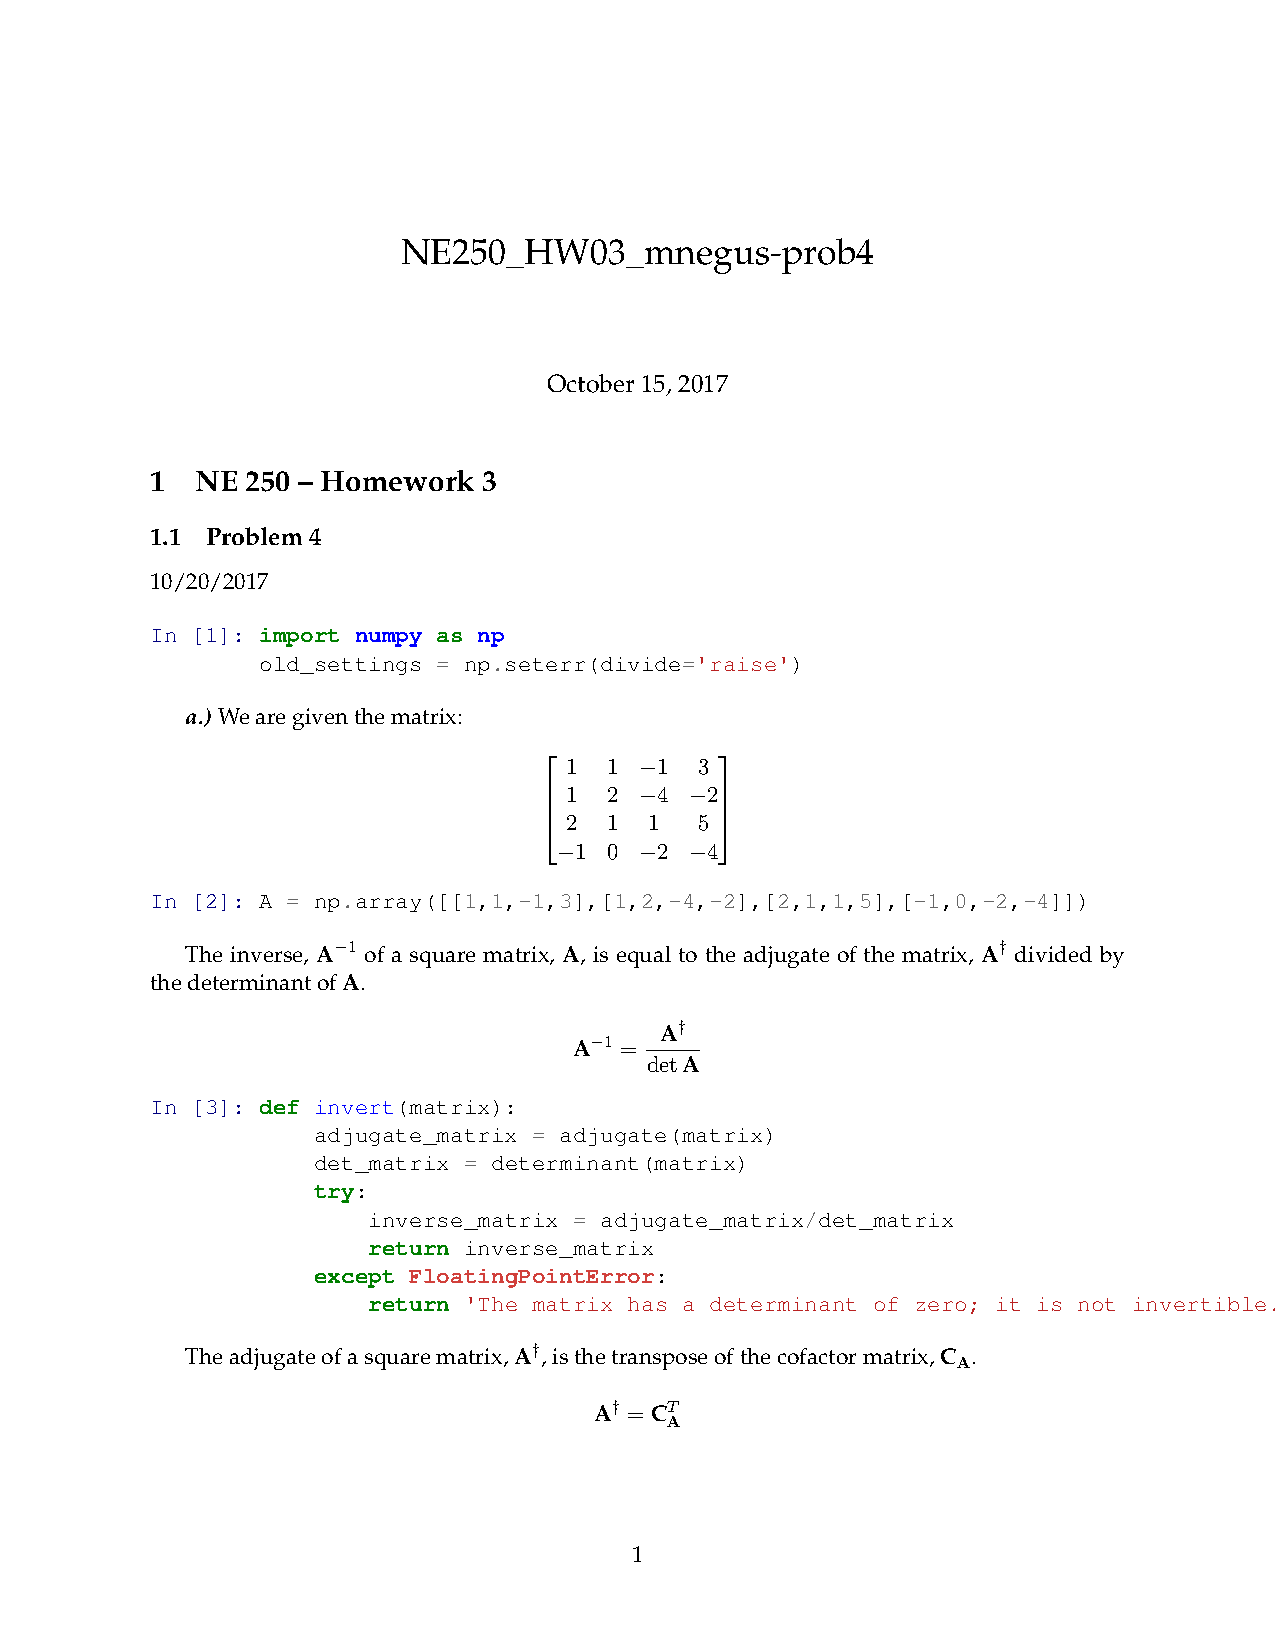
\includepdf[pages=-]{NE250_HW03_mnegus-prob4.pdf}
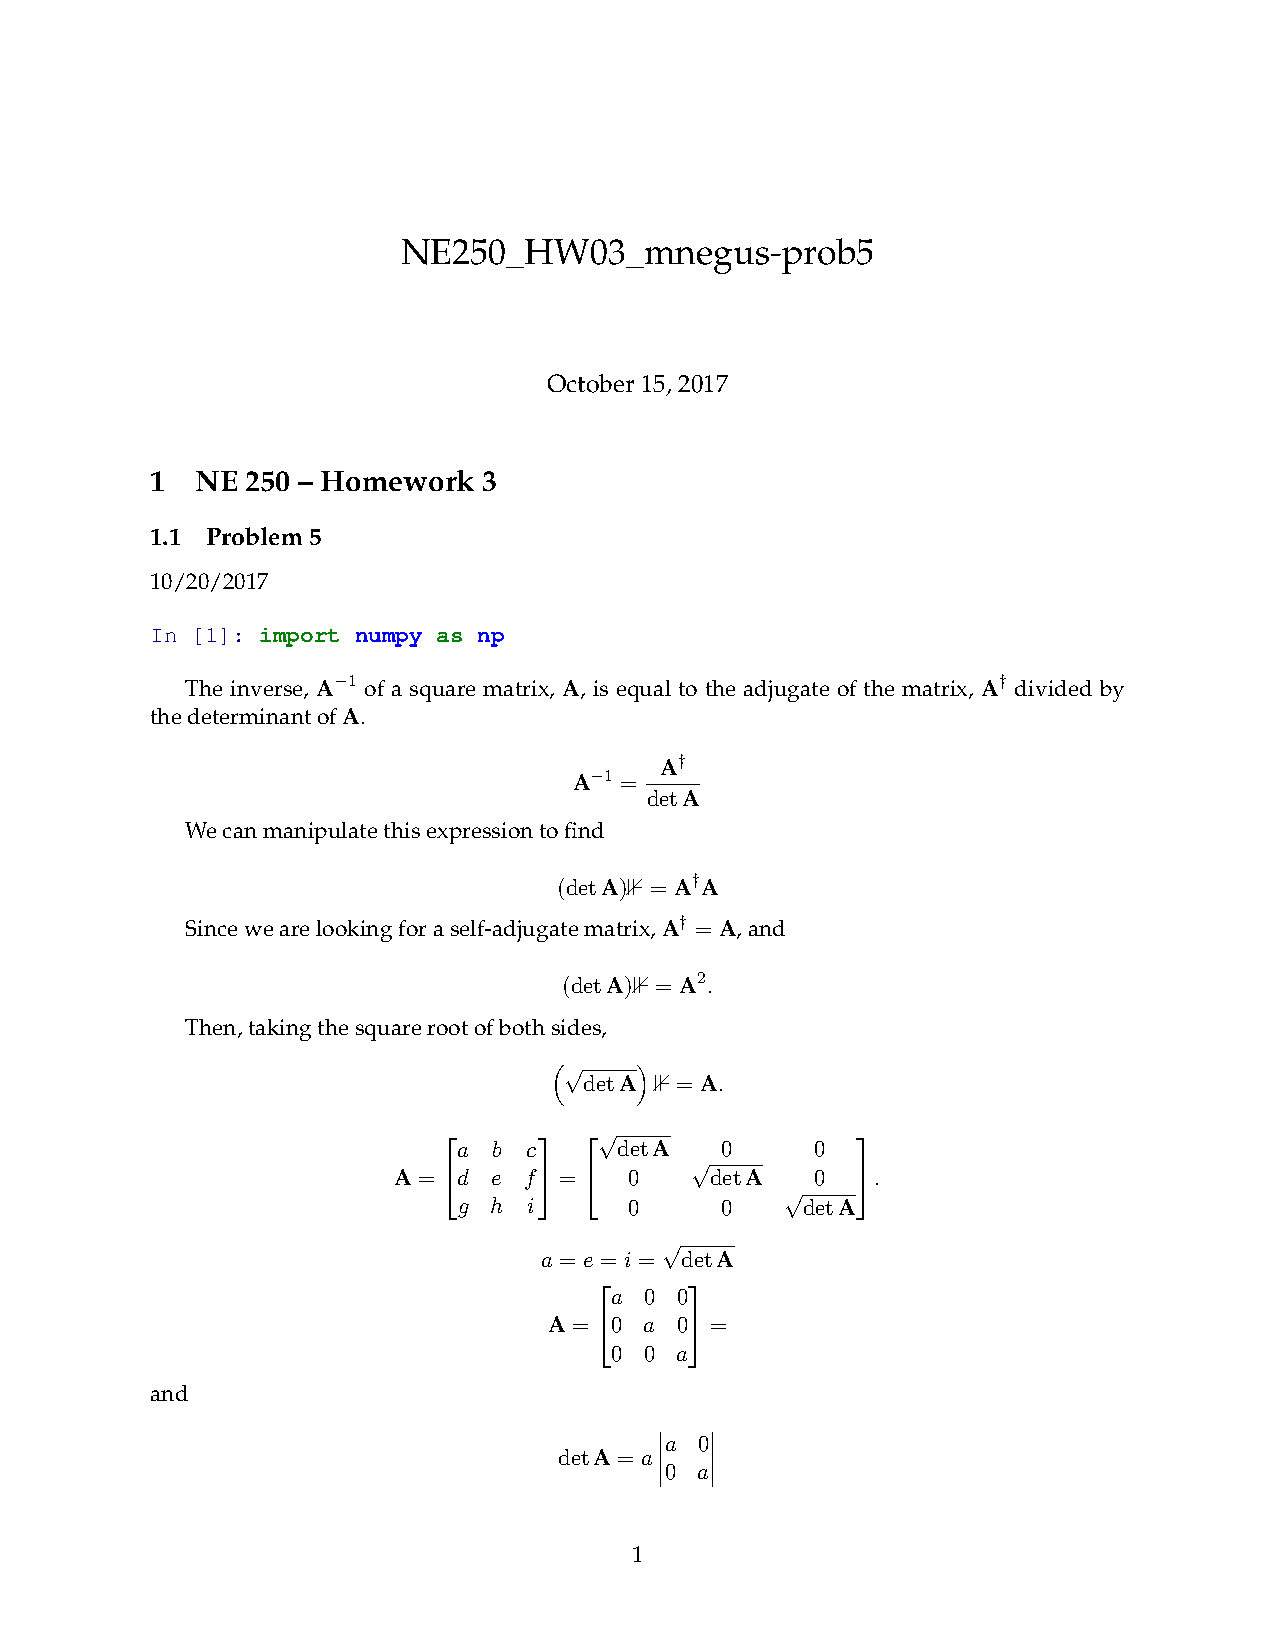
\includepdf[pages=-]{NE250_HW03_mnegus-prob5.pdf}


\end{document}








 
